%\documentclass{article}

%\usepackage[spanish]{babel}
%\usepackage[latin1]{inputenc}
%\usepackage[spanish,activeacute]{babel}

\documentclass[a4paper,10pt]{article}

\usepackage[spanish]{babel}
\usepackage[utf8]{inputenc}
\usepackage{float}
\usepackage{graphicx}


\begin{document}

\section{Optimizaciones.}

\subsection{Inversión de ciclos.}

El método consiste en invertir los ciclos exteriores del método básico. Al realizar la multiplicación A x B = C con el método básico, las matrices A y C se recorren por filas y la B por columnas.
Al intercambiar el orden de los bucles, se cambia el sentido de recorrido de cada matriz, es decir, A y C por columnas y B por filas. Esto permite un mejor aprovechamiento de la localidad espacial que provee la dispocición de los elementos contiguos en la memoria bajo el criterio Column Major Order.


\subsection{Básico con trasposición.}

Como se explico en el m'etodo anterior, A y C se recorren originalmente por filas. Lo que hace este método es transponer A y luego efectuar la multiplicación recorriendo A y B por columnas simultáneamente. Como se utiliza un acumulador para cada elemento de C, se realizan menor cantidad de accesos a éstos últimos, con respecto a los elementos de las otras matrices. Al igual que en el caso anterior, el beneficio se obtiene debido al aprovechamiento de la localidad espacial.

Sin embargo, el desempeño de este método se ve impactado por la penalidad de calcular la matriz traspuesta, porque deben accederse simultáneamente los elementos simétricos respecto a la diagonal (que pertenecen a distintas filas y columnas de la matriz transponer).

\subsection{Multiplicación por bloques}

Es posible dividir la matriz en bloques de tamaño arbitrario y, utilizando el método básico, realizar multiplicaciones sucesivas de matrices mas pequeñas, mejorando la localidad temporal, ya que se mantienen en la caché los datos que se usarán a corto plazo.

\subsection{Multiplicación por columnas.}

Este método realiza la multiplicación de matrices en forma incremental, efectuando todas las operaciones posibles con los elementos disponibles de una de las matrices y sumando los resultados parciales en la matriz resultado.

Utilizando las propiedades de las matrices se consiguen las siguientes equivalencias que proporcionanan fundamento matemático al método. Por simplicidad, se utilizan matrices de 2x2.

$$
  \left[
	\begin{array}{cc}
		a_{11} & a_{12} \\
		a_{21} & a_{22}
	\end{array}
   \right]
   \left[
	\begin{array}{cc}
		b_{11} & b_{12} \\
		b_{21} & b_{22}
	\end{array}
   \right]
   =
   \left[
	\begin{array}{cc}
		c_{11} & c_{12} \\
		c_{21} & c_{22}
	\end{array}
   \right]
$$

El producto del miembro izquierdo se puede escribir como
$$
   \left(
	\left[
	\begin{array}{cc}
		a_{11} & 0 \\
		a_{21} & 0
	\end{array}
	\right]
        +
	\left[
	\begin{array}{cc}
		0 & a_{12} \\
		0 & a_{22}
	\end{array}
	\right]
   \right)
   \left(
   	\left[
	\begin{array}{cc}
		b_{11} & 0 \\
		b_{21} & 0
	\end{array}
	\right]
        +
	\left[
	\begin{array}{cc}
		0 & b_{12} \\
		0 & b_{22}
	\end{array}
	\right]
   \right)
$$

Y expandiendo los paréntesis resulta

$$
	\left[
	\begin{array}{cc}
		a_{11} & 0 \\
		a_{21} & 0
	\end{array}
	\right]
	\left[
	\begin{array}{cc}
		b_{11} & 0 \\
		b_{21} & 0
	\end{array}
	\right]
        +
	\left[
	\begin{array}{cc}
		0 & a_{12} \\
		0 & a_{22}
	\end{array}
	\right]
	\left[
	\begin{array}{cc}
		b_{11} & 0 \\
		b_{21} & 0
	\end{array}
	\right]
	+
	\left[
	\begin{array}{cc}
		a_{11} & 0 \\
		a_{21} & 0
	\end{array}
	\right]
	\left[
	\begin{array}{cc}
		0 & b_{12} \\
		0 & b_{22}
	\end{array}
	\right]
        +
	\left[
	\begin{array}{cc}
		0 & a_{12} \\
		0 & a_{22}
	\end{array}
	\right]
	\left[
	\begin{array}{cc}
		0 & b_{12} \\
		0 & b_{22}
	\end{array}
	\right]
$$

Así, la matriz producto se puede descomponer en la siguiente suma
$$
	\left[
	\begin{array}{cc}
		a_{11} b_{11} & 0 \\
		a_{21} b_{11} & 0
	\end{array}
	\right]
        +
	\left[
	\begin{array}{cc}
		a_{12} b_{21} & 0 \\
		a_{22} b_{21} & 0
	\end{array}
	\right]
	+
	\left[
	\begin{array}{cc}
		0 & a_{11} b_{12} \\
		0 & a_{21} b_{12}
	\end{array}
	\right]
        +
	\left[
	\begin{array}{cc}
		0 & a_{12} b_{22} \\
		0 & a_{22} b_{22}
	\end{array}
	\right]
$$

Como se puede apreciar, las tres matrices se acceden por columnas. Esto resulta en una mejor utilización de la memoria cache.

Para que este método funcione correctamente, se requiere que la matriz donde se almacena el resultado haya sido inicializada en 0. Sin embargo, como esto no es tenido en cuenta en el calculo del tiempo (ya que se realiza para todos los metodos), no presenta una desventaja.

Otro factor importante es el grado de asociatividad de la cache, ya que para que no se produzca trashing tiene que tener como minimo 4 vías para evitar que se reemplacen entre si las columnas de las matrices A, B y C.

Por último, si el tamaño de la matriz a multiplicar es muy grande, las columnas de cada matriz no se pueden mapear completmente en la caché, y si el grado de asociatividad no es el suficiente como para que no se produzcan conflictos no solo entre las matrices, sino también entre las columnas que cada una posee, se puede generar trashing.

\subsection{Multiplicación por columnas, usando operación en bloques}

Este método es la unión de los 2 anteriores, combinando las ventajas de cada uno. Básicamente, con la operacion por bloques se logra reducir el problema que se produce en el método de multiplicación por columnas, al operar con matrices de gran tamaño. Si se escoje el valor adecuado para el tamaño de bloque, se puede lograr operar con matrices pequeñas cuyas columnas entran completamente en cada linea de la caché. De esta manera, se hace un gran aprovechamiento de la localidad espacial y temporal.

\clearpage
\section{Hardware utilizado}

El programa de multiplicación de matrices, con cada optimización implementada, se ejecutó en dos configuraciones de hardware que se describen a continuación.

\subsection{Intel® Pentium® 4 Processor}

\begin{tabular}{|c|c||c|c|}
\hline
\multicolumn{4}{|c|}{Especificaciones} \\
\hline
sSpec Number & SL6PE & Package Type & 478 pin \\
\hline
CPU Speed & 2.66 GHz & Manufacturing Technology & 0.13 micron \\
\hline
PCG & & Core Stepping & D1 \\
\hline
Bus Speed & 533 MHz & CPUID String & 0F29h \\
\hline
Bus/Core Ratio & 20 & Thermal Design Power & 66.1W \\
\hline
L2 Cache Size & 512 KB & Thermal Specification & 74ºC \\
\hline
L2 Cache Speed & 2.66 GHz & VID Voltage Range & 1.53V \\
\hline
\end{tabular}

\begin{verbatim}
Cache Info:
        1st-level data cache: 8 KB, 4-way set associative, sectored cache, 64-byte line size
        Trace cache: 12 K-uops, 8-way set associative
        2nd-level cache: 512 KB, 8-way set associative, sectored cache, 64-byte line size
        Data TLB: 4 KB or 4 MB pages, fully associative, 64 entries
        Instruction TLB: 4 KB, 2 MB or 4 MB pages, fully associative, 128 entries
\end{verbatim}

\subsection{Intel® Core™2 Duo Desktop Processor E6400}

\begin{tabular}{|c|c||c|c|}
\hline
\multicolumn{4}{|c|}{Especificaciones} \\
\hline
sSpec Number  & SL9T9  & Package Type & LGA775 \\
\hline
CPU Speed  & 2.13 GHz  & Manufacturing Technology & 65 nm \\
\hline
PCG  & 06  & Core Stepping & L2 \\
\hline
Bus Speed  & 1066 MHz  & CPUID String & 06F2h \\
\hline
Bus/Core Ratio  & 8  & Thermal Design Power & 65W \\
\hline
L2 Cache Size  & 2 MB & Thermal Specification & 61.4ºC \\
\hline
L2 Cache Speed  & 2.13 GHz & VID Voltage Range & 0.85V  1.5V \\
\hline
\end{tabular}

\begin{verbatim}
Cache Info:
        1st-level data cache: 32 KB, 8-way set associative, 64-byte line size
        1st-level instruction cache: 32 KB, 8-way set associative, 64-byte line size
        2nd-level cache: 2 MB, 8-way set associative, 64-byte line size
        Data TLB: 4 KB Pages, 4-way set associative, 256 entries
        Data TLB: 4 MB Pages, 4-way set associative, 32 entries
        L0 Data TLB: 4 MB pages, 4-way set associative, 16 entries
        L0 Data TLB: 4 MB pages, 4-way set associative, 16 entries
        Instruction TLB: 4 KB Pages, 4-way set associative, 128 entries
        Instruction TLB: 4 MB Pages, 4-way set associative, 4 entries
        Instruction TLB: 2 MB Pages, 4-way set associative, 8 entries
        64-byte Prefetching
\end{verbatim}

\clearpage
\section{Corridas}

\subsection{Intel® Pentium® 4 Processor}

\input{./matmult/pentium4/matmul.salida}
\clearpage
\input{./matmult/pentium4/matmul-3loopi.salida}
\clearpage
\input{./matmult/pentium4/matmul-bloques.salida}
\clearpage
\input{./matmult/pentium4/matmul-lineas.salida}
\clearpage
\input{./matmult/pentium4/matmul-transp.salida}
\clearpage

\subsection{Grafico Comparativo: }
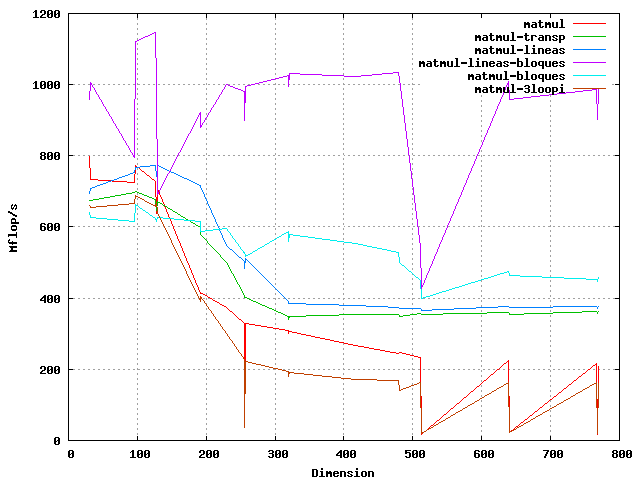
\includegraphics[width=15cm, bb=0 0 640 480]{./pentium4-plot.png}
\clearpage

\subsection{Core 2 Duo E6400}

\input{./matmult/core2/matmul.salida}
\clearpage
\input{./matmult/core2/matmul-3loopi.salida}
\clearpage
\input{./matmult/core2/matmul-bloques.salida}
\clearpage
\input{./matmult/core2/matmul-lineas.salida}
\clearpage
\input{./matmult/core2/matmul-transp.salida}
\clearpage
\input{./matmult/core2/matmul-lineas-bloques.salida}
\clearpage

\subsection{Grafico Comparativo: }

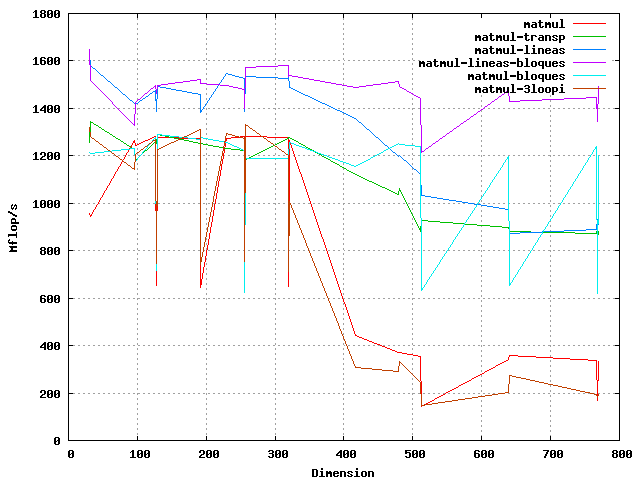
\includegraphics[width=15cm, bb=0 0 640 480]{core2-plot.png}
\clearpage

\section{Analisis de resultados y conclusiones: }

\subsection{Inversión de ciclos.}

Como se observa en los gráficos, el multiplicar básico es muy inestable respecto del tamaño de matriz utilizado y el más ineficiente. Asimismo, lo único que produce la mejora propuesta es un \textbf{pequeño} aumento de la estabilidad y del rendimiento. La curva mantiene la misma tendencia que la del método básico.

\subsection{Básico con trasposición.}

En este caso podemos notar que el método es bastante estable (en contraposición con los anteriores).

Cuando la matriz es pequeña, el costo de transposición es pequeño, y la ventaja de recorrer por columnas no se ve tan perjudicada, obteniendo un buen desempeño. 

Cuando la matrices a multiplicar son muy grandes, este método presenta 2 problemas: Por un lado el costo de transposición aumenta, porque los elementos simétricos están más separados en memoria y se pierde localidad espacial, y por el otro lado, cada columna columna sobrepasa el tamaño de la caché y se genera trashing. Este fenómeno se puede apreciar en el gráfico (con la brusca caída de mflops alrededor de un tamaño identificable).

\subsection{Multiplicación por columnas.}

Se puede ver que este método se comporta de manera similar al anterior (porque se basan en el mismo principio) sin el tiempo consumido por el proceso de transposición, por lo que la curva mflops(tamaño) se encuentra desplazada hacia arriba.

\subsection{Multiplicación por bloques.}

Este método evidencia la ventaja de trabajar con matrices de un tamaño deseado (pudiendo elegir el mas conveniente para cada situación).

El desempeño es muy variable y depende de la compatibilidad entre las dimensiones de las matrices y el tamaño del bloque (sin dejar de lado el tamaño de la cache y el grado de asociatividad de la misma). Esto significa que se puede lograr un gran rendimiento al procesar matrices muy grandes, eligiendo correctamente el bloque, cosa que no se puede realizar con los otros métodos. 

Todo esto esto se puede ver claramente en el gráfico.

\subsection{Multiplicación por columnas y bloques.}

Como supusimos, se logran aprovechar las ventajas de los dos métodos anteriores. 

Se pudo elegir el tamaño de bloque de manera tal de operar la mayor parte del tiempo con matrices que povocan un rendimiento óptimo para el método de multiplicación por columnas. De esta manera se logra mantener este nivel sin importar el tamaño de la matriz original.

\clearpage
\section{Código fuente}

\end{document}
